\section{Definicje}

\subsection*{Graf ogólny, graf prosty}

\textbf{Graf} (\textbf{graf ogólny}, \textbf{multigraf}) $G$ jest parą $(V(G),E(G))$, gdzie $V(G)$ jest skończonym, niepustym zbiorem elementów zwanych \textbf{wierzchołkami}, a $E(G)$ jest skończoną rodziną nieuporządkowanych par elementów zbioru $V(G)$ zwanych \textbf{krawędziami} \cite[20]{wilson} (tj. $E(G) \subseteq \{\{u,v\} : u,v \in V(G)\}$). Zbiór $V(G)$ nazywamy zbiorem wierzchołków, a rodzinę $E(G)$ -- \textbf{rodziną krawędzi} grafu $G$; gdy nie ma możliwości pomyłki często są skracane do odpowiednio $V$ oraz $E$. (Niektóre definicje nie wymagają, aby zbiory $V$ oraz $E$ były skończone \cite[143]{ross}, ale ponieważ w naszych zastosowaniach będziemy mieli do czynienia ze zbiorami skończonymi, przyjmiemy, że zbiory te są skończone).  Wierzchołki $u,v \in V$ są \textbf{połączone} krawędzią $\{u,v\}$ (lub krócej $uv$), gdy $\{u,v\} \in E$. 

Zauważmy, że taka definicja dopuszcza sytuację, w której dwa wierzchołki są połączone więcej niż jedną krawędzią (tzw. \textbf{krawędź wielokrotna}) oraz gdy wierzchołek jest połączony z samym sobą (tzw. \textbf{pętla}). Graf, który nie posiada krawędzi wielokrotnych oraz pętli nazywamy \textbf{grafem prostym} \cite[19]{wilson}.

\begin{figure}[h]
\centering
\begin{minipage}{.45\textwidth}
  \centering
  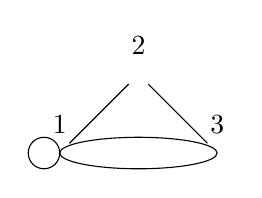
\begin{tikzpicture}
\filldraw 
(0,0) node[label=1](1){}
(1,1) node[label=2](2){} 
(2,0) node[label=3](3){};
\draw (0,0) arc (0:360:2mm);
\draw (2,0) arc (0:180:1 and 0.2);
\draw (0,0) arc (180:360:1 and 0.2);
\path[draw] (1)--(2);
\path[draw] (2)--(3);
\end{tikzpicture}
\captionsetup{justification=centering}
\caption{Przykład grafu~ogólnego} \label{fig:simple-graph}
\end{minipage}
\begin{minipage}{.45\textwidth}
  \centering
  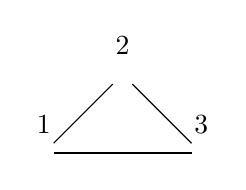
\begin{tikzpicture}
\filldraw 
(0,0) node[label=1](1){}
(1,1) node[label=2](2){} 
(2,0) node[label=3](3){};
\path[draw] (1)--(2);
\path[draw] (2)--(3);
\path[draw] (3)--(1);
\end{tikzpicture}
\captionsetup{justification=centering}
\caption{Przykład grafu~prostego} \label{fig:graph}
\end{minipage}
\end{figure}


\subsection*{Sąsiedztwo}

Wierzchołki $u,v \in V$ są \textbf{sąsiednie} jeśli istnieje krawędź $uv$ (wówczas wierzchołki $u$ i $v$ są \textbf{incydentne} z tą krawędzią). Dwie krawędzie są \textbf{sąsiednie}, jeśli są incydentne z tym samym wierzchołkiem. 

\textbf{Stopień} wierzchołka $v \in V$ (oznaczany jako $deg(v)$) jest liczbą krawędzi incydentnych z $v$. \textbf{Wierzchołek izolowany} to wierzchołek stopnia 0, a \textbf{wierzchołek końcowy} -- stopnia 1.

Istnieją dwie standardowe reprezentacje grafów w pamięci komputera: jako \textbf{listy sąsiedztwa} lub jako \textbf{macierze sąsiedztwa} \cites[29]{banachowski}[600]{cormen}. Pierwsza z nich polega na zapamiętaniu dla każdego wierzchołka listy wierzchołków z nim sąsiadujących. Druga zakłada, że wierzchołki są ponumerowane liczbami ze zbioru $\{1, 2,\ldots,n\}$ (gdzie $n$ oznacza moc zbioru $V$) i opiera się na stworzeniu macierzy wymiaru $n \times n$, której wyraz o indeksach $i,j$ jest równy liczbie krawędzi łączących wierzchołek o numerze $i$ z wierzchołkiem o numerze $j$.

Innym sposobem reprezentacji grafu za pomocą macierzy jest \textbf{macierz incydencji}. Jeśli krawędzie oznakujemy liczbami ze zbioru $\{1,2,\ldots,m\}$ (gdzie $m$ moc zbioru $E$), to jest to macierz o rozmiarze $n \times m$, której wyraz o indeksach $i,j$ jest równy 1, jeśli wierzchołek z numerem $i$ jest incydentny z krawędzią $j$, i jest równy 0 w przeciwnym przypadku \cite[27]{ross}.

\begin{figure}[H]
\centering
  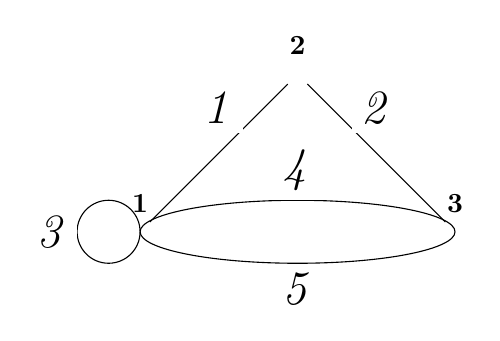
\begin{tikzpicture}
\filldraw 
(0,0) node[label=\textbf{1}](1){}
(2,2) node[label=\textbf{2}](2){} 
(4,0) node[label=\textbf{3}](3){};
\draw (0,0) arc (0:360:4mm) node [midway,left,fill=white] {\LARGE\textit{3}};
\draw (4,0) arc (0:180:2 and 0.4) node [midway,above,fill=white] {\LARGE\textit{4}};;
\draw (0,0) arc (180:360:2 and 0.4) node [midway,below,fill=white] {\LARGE\textit{5}};;
\path[draw] (1)--(2) node [midway,above=7pt,fill=white] {\LARGE\textit{1}};
\path[draw] (2)--(3) node [midway,above=7pt,fill=white] {\LARGE\textit{2}};
\end{tikzpicture}
\caption{}\label{fig:graph-edge-labeled}
\end{figure}

Macierz sąsiedztwa $A$ i macierz incydencji $M$ dla grafu z rysunku \ref{fig:graph-edge-labeled}:

\[A = 
 \begin{pmatrix}
  1 & 1 & 2 \\
  1 & 0 & 1 \\
  2 & 1 & 0 
 \end{pmatrix}, \hspace{20pt}
 M = 
 \begin{pmatrix}
  1 & 0 & 1 & 1 & 1 \\
  1 & 1 & 0 & 0 & 0 \\
  0 & 1 & 0 & 1 & 1 
 \end{pmatrix}
\]


\subsection*{Podgraf}
\textbf{Podgraf} $G'=(V',E')$ grafu $G=(V,E)$ to graf, którego wszystkie wierzchołki nalezą do $V$, a krawędzie należą do $E$ (tj. $V' \subseteq V$ oraz $E' \subseteq E$).Jeśli $V' = V$, to podgraf $G'$ nazywany jest \textbf{podgrafem rozpinającym} \cite[229]{banachowski}. 

Podgraf jest \textbf{indukowany} przez $V'$, jeśli zawiera wszystkie krawędzie z grafu $G$ o końcach w wierzchołkach z $V'$ (tj. $E'=\{(u,v) \in E: u,v \in V' \}$) \cite[1195]{cormen}.


\subsection*{Trasa, ścieżka, droga, cykl}

\textbf{Trasa} w grafie $G$ to skończony ciąg krawędzi $v_0v_1,v_1v_2\ldots v_{m-1}v_m$ (zapisywany również w postaci $v_0 \rightarrow v_1 \rightarrow \ldots \rightarrow v_m$), w którym każde dwie kolejne krawędzie są albo sąsiednie, albo identyczne \cite[41]{wilson}. Trasa wyznacza ciąg wierzchołków $v_0,v_1,\ldots,v_m$ -- pierwszy z nich nazywamy \textbf{wierzchołkiem początkowym}, a ostatni \textbf{wierzchołkiem końcowym}. Liczba krawędzi na trasie to \textbf{długość trasy}. 

\textbf{Ścieżka} to trasa, w której wszystkie krawędzie są różne. Jeśli również wszystkie wierzchołki $v_0,v_1,\ldots,v_m$ są różne (dopuszczając jedynie możliwość, aby wierzchołek początkowy był równy wierzchołkowi końcowemu), to ścieżka nazywana jest \textbf{drogą}. Droga (lub ścieżka) jest \textbf{zamknięta}, jeśli $v_0 = v_m$; ścieżka zamknięta, która posiada co najmniej jedną krawędź to \textbf{cykl}; droga zamknięta, która posiada co najmniej jedną krawędź to \textbf{cykl prosty}.

Jeśli istnieje ścieżka z $u$ do $v$, to mówimy, że $v$ jest \textbf{osiągalny} z $u$.


\subsubsection*{Cykl Eulera}

\textbf{Cykl Eulera} to taki cykl w grafie, który przechodzi przez każdą jego krawędź dokładnie jeden raz. Graf spójny, który posiada cykl Eulera nazywany jest \textbf{grafem eulerowskim}. 

\begin{theorem}[Euler, 1736]
Graf spójny $G$ jest grafem eulerowskim wtedy i tylko wtedy, gdy stopień każdego wierzchołka grafu $G$ jest liczbą parzystą.
\end{theorem}

\begin{theorem}
Skierowany graf spójny $G$ jest eulerowski wtedy i tylko wtedy, gdy każdy wierzchołek grafu $G$ ma tyle samo krawędzi wchodzących i wychodzących.
\end{theorem}


\subsubsection*{Cykl Hamiltona}

\textbf{Cykl Hamiltona} to taki cykl w grafie, który przechodzi przez każdy jego wierzchołek dokładnie jeden raz. Graf spójny posiadający cykl Hamiltona nazywany jest \textbf{grafem hamiltonowskim}.

W przeciwieństwie do problemu stwierdzenia czy graf jest eulerowski, nie jest znany warunek konieczny i wystarczający na to, aby graf był hamiltonowksi. Problem stwierdzania czy graf jest hamiltonowski należy do jednych z najważniejszych nierozwiązanych problemów teorii grafów \cite[54]{wilson}. 

Istnieją twierdzenia (np. Twierdzenie \ref{theorem:dirac}, \ref{theorem:orego}), które na podstawie cech grafu pozwalają stwierdzić, czy graf jest hamiltonowski. Mają one postać: ,,jeśli graf ma wystarczająco dużo krawędzi, to ma cykl Hamiltona'' \cite[54]{wilson}. Są to jednak implikacje jednostronne -- istnieją grafy hamiltonowskie, które nie spełniają poprzedników tych implikacji. 

\begin{theorem}[Dirac, 1952]\label{theorem:dirac}
Jeśli w grafie prostym $G$, który ma $n$ wierzchołków (gdzie $n \geq 3$)
\[deg(v) \geq \frac{n}{2}\] 
dla każdego wierzchołka $v$, to graf $G$ jest hamiltonowski.
\end{theorem}

\begin{theorem}[Orego, 1960]\label{theorem:orego}
Jeśli graf prosty $G$ ma $n$ wierzchołków (gdzie $n\geq 3$), oraz
\[
deg(v) + deg(w) \geq n
\]
dla każdej pary wierzchołków niesąsiednich $v$ i $w$, to graf $G$ jest hamiltonowski.
\end{theorem}


\subsection*{Graf skierowany}

\textbf{Graf skierowany}, \textbf{digraf} (ang. \textit{directed graph}) $G$ to para $(V(G),\ E(G))$, gdzie $V(G)$ niepusty, skończony zbiór elementów zwanych \textbf{wierzchołkami}, a $E(G)$ skończony zbiór par \emph{uporządkowanych} elementów ze zbioru $V(G)$ zwanych \textbf{krawędziami} (lub \textbf{łukami} \cite[135]{wilson}). Digraf $G$ jest \textbf{digrafem prostym}, jeśli wszystkie krawędzie są różne oraz jeśli nie posiada pętli. 

Jeśli $e = (v,w) \in E(G)$, to $v$ nazywamy \textbf{początkiem krawędzi} $e$, a $w$ -- \textbf{końcem krawędzi} $e$.

Definicje z poprzedniej podsekcji w naturalny sposób uogólniają się na przypadek digrafów \cite[136]{wilson}. 


\subsection*{Spójność}

Załóżmy, że mamy dwa grafy $G_1 = (V_1,E_1)$ oraz $G_2 = (V_2,E_2)$, gdzie $V_1 \cap V_2 = \emptyset$. Wówczas \textbf{sumą} tych grafów $G_1 \cup G_2$ jest graf $G=(V_1\cup V_2, E_1\cup E_2)$. Graf nazywamy \textbf{spójnym}, jeśli nie można przedstawić go w postaci sumy dwóch grafów, w przeciwnym razie graf jest \textbf{niespójny} \cite[22]{wilson}. Każdy graf niespójny $G$ możemy przedstawić jako sumę grafów spójnych, nazywanych \textbf{spójnymi składowymi} grafu $G$ (rysunek \ref{fig:connected-copoments-example} przedstawia graf posiadający dwie spójne składowe). 

\begin{figure}[h]
\centering
\begin{tikzpicture}
\filldraw 
(0,0) node(1){}
(1,1) node(2){} 
(2,0) node(3){}
(4,0) node(4){}
(4,1) node(5){};
\path[draw] (1)--(2);
\path[draw] (2)--(3);
\path[draw] (3)--(1);
\path[draw] (4)--(5);
\end{tikzpicture}
\caption{Przykład grafu mającego dwie spójne składowe} \label{fig:connected-copoments-example}
\end{figure}

Niektórzy autorzy \cite[342]{ross} podają alternatywną, równoważną \cite[42]{wilson} definicję grafu spójnego -- jest to graf, w którym każda para różnych wierzchołków jest połączona drogą. 

Graf skierowany $G$ jest \textbf{silnie spójny}, jeśli dla dowolnych dwóch wierzchołków $v$ i $w$ istnieje droga z $v$ do $w$. Każdy digraf silnie spójny jest spójny, ale nie wszystkie digrafy spójne są silnie spójne. 

\textbf{Dwuspójną składową} grafu $G$ nazywamy maksymalny podzbiór krawędzi, taki że każde dwie krawędzie z tego zbioru leżą na wspólnym cyklu prostym \cite[634]{cormen}. W dwuspójnej składowej pomiędzy każdą parą wierzchołków istnieją dwie rozłączne krawędziowo drogi. Wierzchołki należące do co najmniej dwóch różnych dwuspójnych składowych nazywamy \textbf{wierzchołkami rozdzielającymi} (lub \textbf{punktami artykulacji} \cite[633]{cormen}). Usunięcie wierzchołka rozdzielającego ,,rozspójnia'' graf. Krawędzie, które nie należą do żadnego cyklu prostego nazywamy \textbf{mostami}. Ich usunięcie również ,,rozspójnia'' graf.

Graf, który posiada tylko jedną dwuspójną składową nazywamy \textbf{grafem dwuspójnym} \cite[232]{banachowski}.

\begin{figure}[H]
\centering
\begin{tikzpicture}
\fill[fill=light-gray] (1,0) -- (0,1) -- (1,2) -- (2,1);
\filldraw 
(1,0) node[color=gray](1){}
(0,1) node[color=gray](2){} 
(2,1) node(3){}
(1,2) node[color=gray](4){};
\path[draw,color=gray] (1)--(2);
\path[draw,color=gray] (2)--(3);
\path[draw,color=gray] (3)--(4);
\path[draw,color=gray] (4)--(1);
\path[draw,color=gray] (1)--(3);
\path[draw,color=gray] (2)--(4);

\fill[fill=light-gray] (5,0) -- (4,1) -- (5,2);
\filldraw 
(5,0) node[color=gray](5){}
(4,1) node(6){} 
(5,2) node[color=gray](7){};
\path[draw,color=gray] (5)--(6);
\path[draw,color=gray] (6)--(7);
\path[draw,color=gray] (7)--(5);
\path[draw] (3)--(6);
\end{tikzpicture}
\captionsetup{justification=centering}
\caption{Przykład grafu zawierającego trzy dwuspójne składowe -- punkty artykulacji i mosty zostały zaznaczone na czarno.} \label{fig:biconnected-copoments-example}
\end{figure}


\subsection*{Drzewo, las, drzewo rozpinające}

\textbf{Drzewo} to graf spójny nie posiadający cykli. \textbf{Las} to graf, którego spójnymi składowymi są drzewa.

Drzewem rozpinającym graf $G$ nazywamy podgraf rozpinający $G$, który nie zawiera cykli \cite[10]{wilson-beineke}. 

\begin{figure}[h]
\centering
\begin{tikzpicture}
\filldraw 
(0,0) node(1){}
(1,1) node(2){} 
(2,0) node(3){}
(2,2) node(4){}
(3,1) node(5){};
\path[draw] (1)--(2);
\path[draw] (2)--(3);
\path[draw] (2)--(4);
\path[draw] (4)--(5);
\end{tikzpicture}
\caption{Przykład grafu będącego drzewem} \label{fig:tree-example}
\end{figure}


\subsection*{Planarność}

\textbf{Graf planarny} to graf, który można narysować na płaszczyźnie tak, aby żadne dwie krzywe obrazujące krawędzie nie przecinały się ze sobą. Odwzorowanie grafu na płaszczyźnie o tej własności nazywane jest \textbf{rysunkiem płaskim} (lub \textbf{grafem płaskim}) \cite[82]{wilson}. 

Na rysunku \ref{fig:planar-graph-example} jest narysowany na dwa sposoby graf pełny $K_4$ (opisany w następnej sekcji \ref{sec:common-graphs}) -- drugi sposób jest przykładem rysunku płaskiego. 

\begin{figure}[h]
\centering
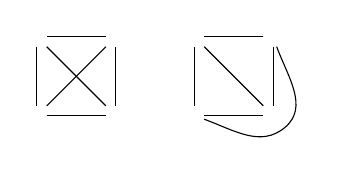
\begin{tikzpicture}
\filldraw 
(0,0) node(1){}
(1,0) node(2){} 
(1,1) node(3){}
(0,1) node(4){};
\path[draw] (1)--(2);
\path[draw] (2)--(3);
\path[draw] (3)--(4);
\path[draw] (4)--(1);
\path[draw] (2)--(4);
\path[draw] (1)--(3);
\filldraw 
(2,0) node(5){}
(3,0) node(6){} 
(3,1) node(7){}
(2,1) node(8){};
\path[draw] (5)--(6);
\path[draw] (6)--(7);
\path[draw] (7)--(8);
\path[draw] (8)--(5);
\path[draw] (6)--(8);
\draw [-] (5) to [out=-20,in=-140] (3.15,-0.15) to [out=40, in=-70 ] (7);
\end{tikzpicture}
\caption{$K_4$ -- przykład grafu planarnego} \label{fig:planar-graph-example}
\end{figure}


\subsection*{Kolorowanie}

\subsubsection*{Kolorowanie wierzchołków}

Jeśli graf $G$ nie ma pętli oraz jeśli każdemu wierzchołkowi możemy przypisać jeden z $k$ kolorów w taki sposób, aby sąsiednie wierzchołki miały różne kolory, to graf G jest grafem \textbf{$k$-kolorowalnym}. Jeśli graf $G$ jest $k$-kolorowalny, ale nie jest $(k-1)$-kolorowalny, to mówimy, że jest \textbf{$k$-chromatyczny} lub że jego \textbf{liczba chromatyczna} wynosi $k$.  

\subsubsection*{Kolorowanie krawędzi}

Jeśli krawędzie grafu $G$ możemy pokolorować $k$ kolorami w taki sposób, aby żadne dwie sąsiednie krawędzie nie miały tego samego koloru, to graf $G$ jest \textbf{$k$-kolorowalny krawędziowo}. Jeśli graf $G$ jest $k$-kolorowalny krawędziowo, ale nie jest $(k-1)$-kolorowalny krawędziowo, to mówimy, że $G$ ma \textbf{indeks chromatyczny} równy $k$.


\subsection*{Skojarzenia}

\textbf{Skojarzeniem} w grafie $G=(V,E)$ nazywamy taki podzbiór krawędzi $M \subseteq E$, w którym żadne dwie krawędzie nie są ze sobą sąsiadujące. Wierzchołek $v \in V$ jest \textbf{skojarzony} w podzbiorze $M$, jeśli pewna krawędź z $M$ jest incydentna z $v$. Skojarzenie jest \textbf{doskonałe} (lub \textbf{całkowite}), jeśli każdy wierzchołek jest skojarzony.

Poniższe twierdzenie podaje warunek konieczny i wystarczający, aby dany graf dwudzielny posiadał skojarzenie doskonałe.

\begin{theorem}[Hall, 1935]\label{theorem:hall}
W grafie dwudzielnym $G=(V_1 \cup V_2, E)$, w którym $|V_1|=|V_2|$ istnieje skojarzenie doskonałe wtedy i tylko wtedy, gdy dla każdego podzbioru $K \subseteq V_1$ zachodzi 
\[|K| \leq |N(K)|,\quad \text{gdzie } N(K)=\{ w \in V_2: \exists_{k \in K} \{k,w\} \in E \}\]
\end{theorem}
